\section{7th Sheaf Cobordism}
Suppose we have a punctured Riemann sphere $M$ and $\Lambda_0^0$, $\Lambda_0^\infty$, $\Lambda_0^{squig}$, a nested regions $U\subset U' \subset M$, and a chart $f : U \rightarrow \R^2$ such that $U'$ maps to $R:=(-1,1)_x \times (0,n+1)_z$ under $f$
\begin{itemize}
\item $\Lambda_0^0$ gets mapped to $\{(x,z)\in R \mid z=\Psi(\frac{1}{2},n+\frac{1}{2})(x)\}$, co-oriented upward.

\item $\Lambda_0^\infty$ gets mapped to $\overset{n}{\underset{k=1}{\cup}}\{(x,z)\in R \mid z=-k\}$, co-oriented downward.

\item $\Lambda_0^{squig}$ gets mapped to $\phi$.
\end{itemize}
and a sheaf defined by the following squiggly legible diagram. All the maps corresponding to blue strands are $\iota_1$ and the red strands $\iota_0$ otherwise stated. I have omitted these maps from the diagram.\\

\begin{figure}[H]
    \centering
    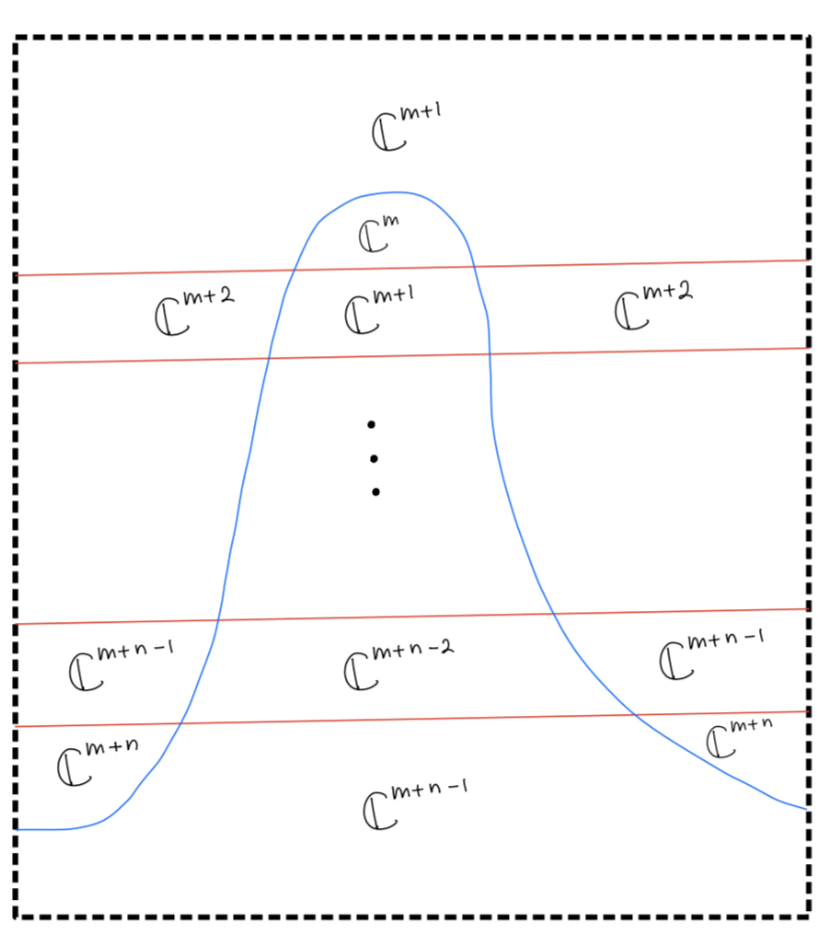
\includegraphics[scale = 0.95]{diagrams/cobord7/1.png}
    \caption{}
    \label{fig:your-label}
\end{figure}

Then we define a cobordism starting from the above sheaf, say $cobord_5(n)$ supported on $U$, where $n$ is the number of red strands. At the end of the cobordism , the sheaf, under the same chart $f$, is described as the following squiggly legible diagram.
\begin{figure}[H]
    \centering
    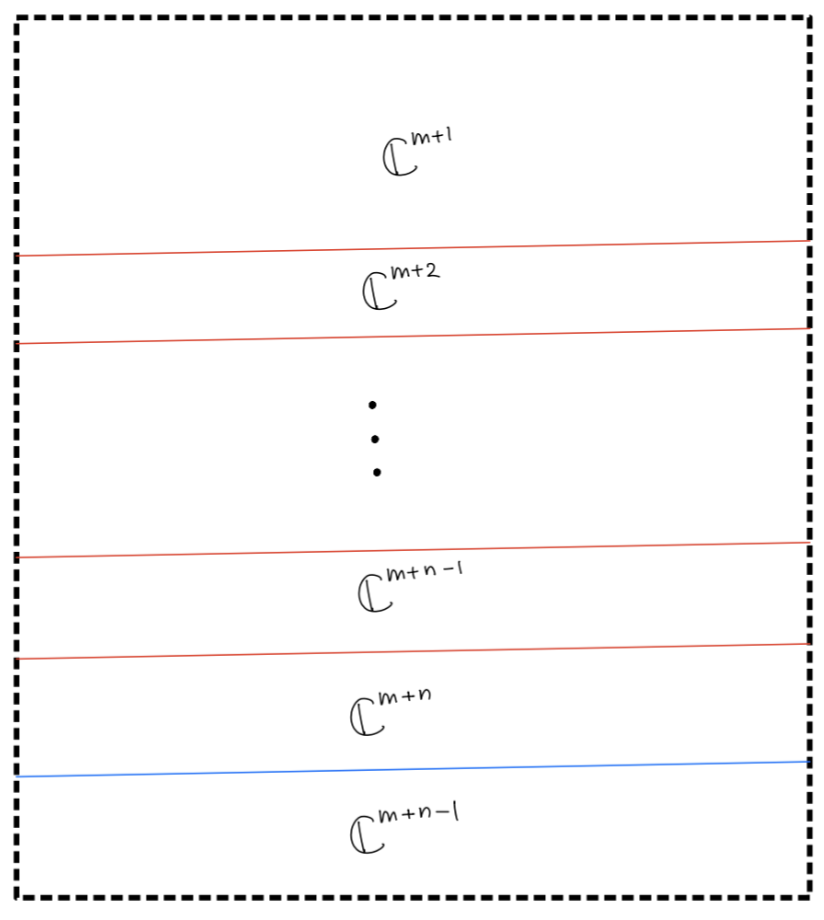
\includegraphics[scale = 0.95]{diagrams/cobord7/7.png}
    \caption{}
    \label{fig:your-label}
\end{figure}

We define $cobord_7(n)$ inductively as follows.
\begin{enumerate}[label=(\roman*)]
\item For $n=1$, we define $cobord_7(1)$ to be $cobord_3$ from
\begin{figure}[H]
    \centering
    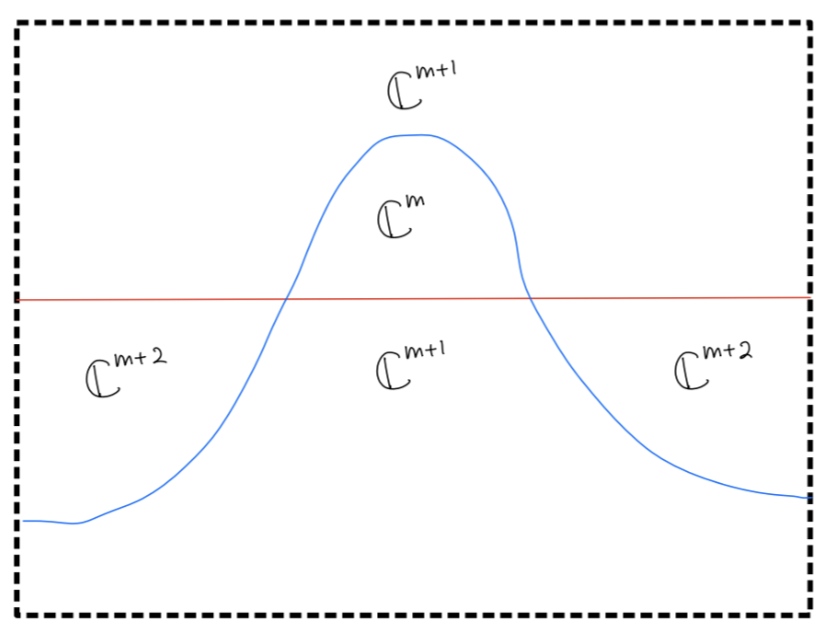
\includegraphics[scale = 0.95]{diagrams/cobord7/2.png}
    \caption{}
    \label{fig:your-label}
\end{figure}
to
\begin{figure}[H]
    \centering
    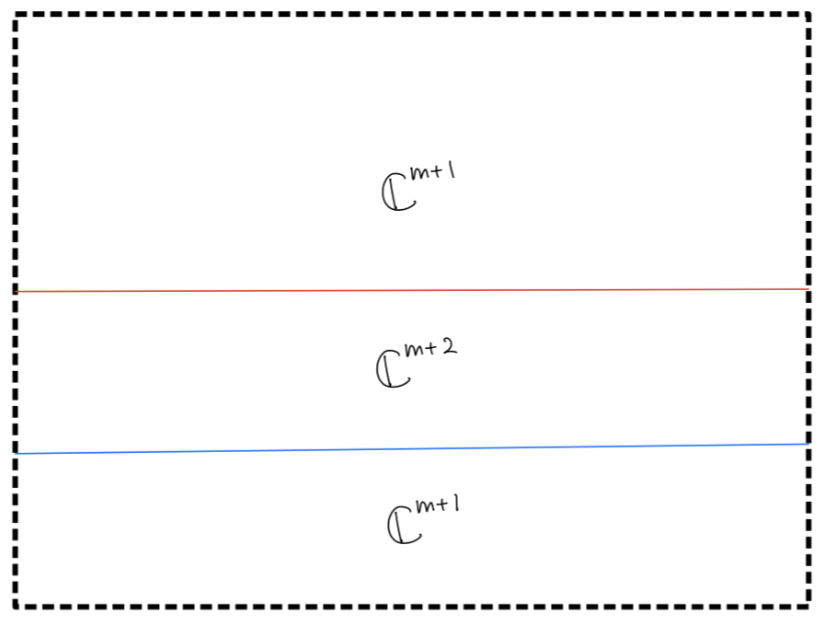
\includegraphics[scale = 0.95]{diagrams/cobord7/3.png}
    \caption{}
    \label{fig:your-label}
\end{figure}

\item For $n>0$,
\begin{enumerate}[label=(Step \arabic*)]
\item we first apply $cobord_7(n-1)$ to the square region surrounded by purple dotted lines.

\begin{figure}[H]
    \centering
    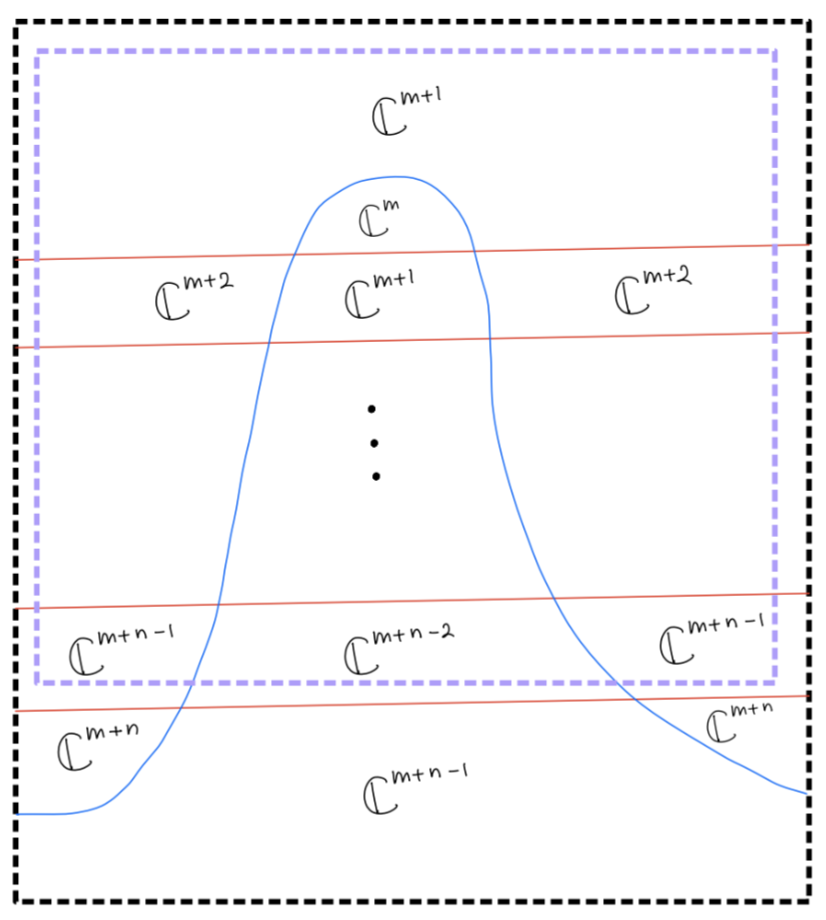
\includegraphics[scale = 0.95]{diagrams/cobord7/4.png}
    \caption{}
    \label{fig:your-label}
\end{figure}

by induction hypothesis, we get

\begin{figure}[H]
    \centering
    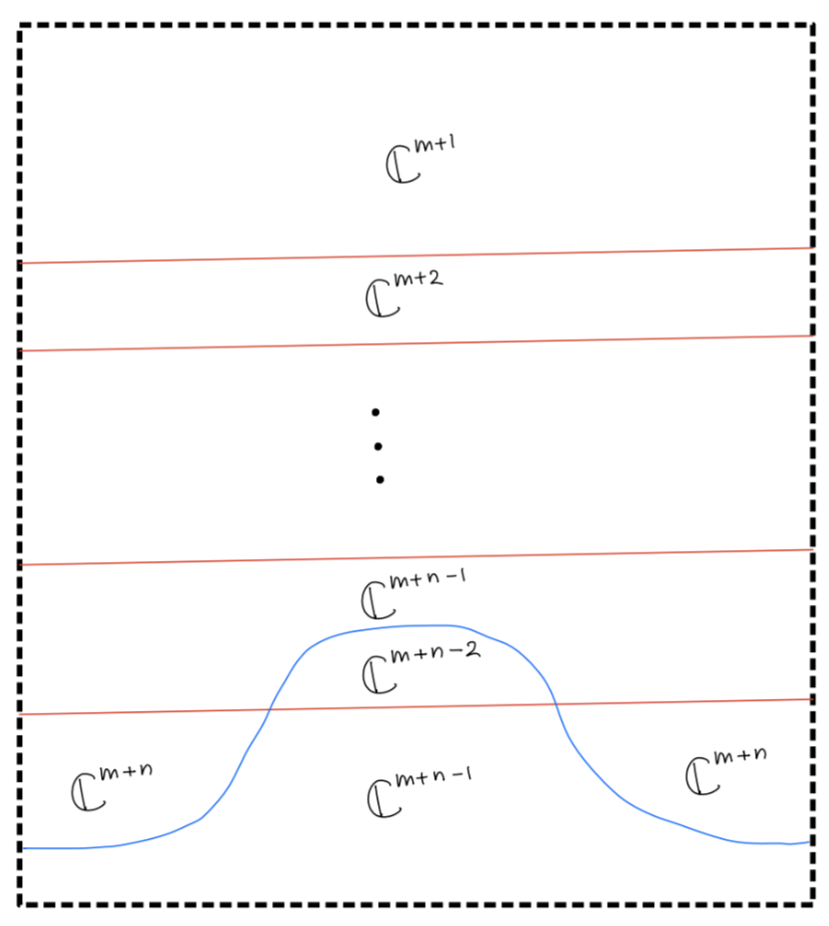
\includegraphics[scale = 0.95]{diagrams/cobord7/5.png}
    \caption{}
    \label{fig:your-label}
\end{figure}

\item apply $cobord_3$ to the square region surrounded by purple dotted lines.

\begin{figure}[H]
    \centering
    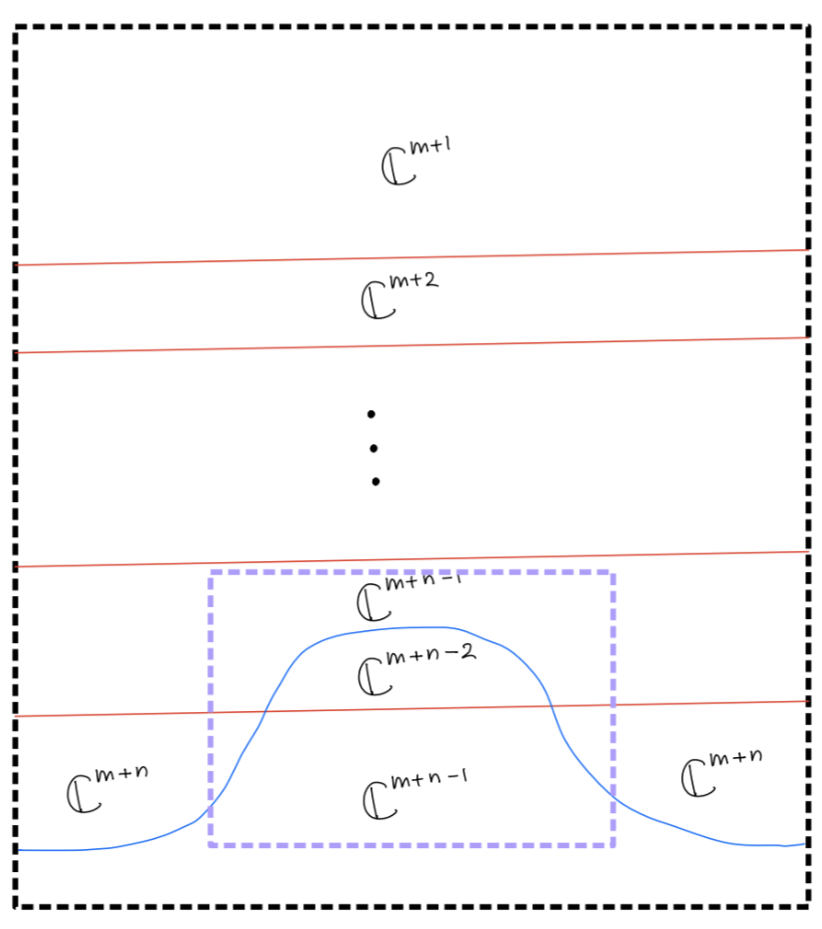
\includegraphics[scale = 0.95]{diagrams/cobord7/6.png}
    \caption{}
    \label{fig:your-label}
\end{figure}

we get the final sheaf

\begin{figure}[H]
    \centering
    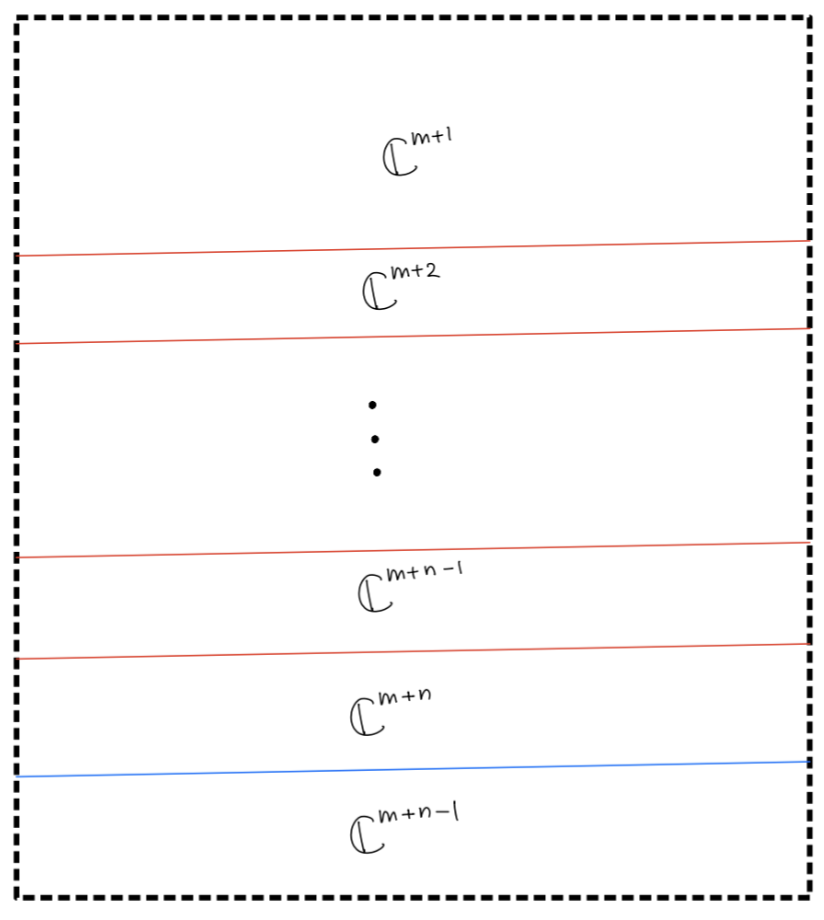
\includegraphics[scale = 0.95]{diagrams/cobord7/7.png}
    \caption{}
    \label{fig:your-label}
\end{figure}
\end{enumerate}
\end{enumerate}